\documentclass[aspectratio=169, 11pt]{beamer}
\usetheme{Madrid}
\usecolortheme{beaver}
\setbeamertemplate{navigation symbols}{}
\setbeamertemplate{footline}[frame number]

\usepackage{amsmath,amssymb}
\usepackage{graphicx}
\graphicspath{{../figures/}}
\usepackage{booktabs}

% ── Colours ───────────────────────────────────────────────────────────────────
\definecolor{mblue}{RGB}{30,100,180}
\definecolor{mred}{RGB}{180,30,30}
\definecolor{mgreen}{RGB}{30,140,60}

% ── Title info ────────────────────────────────────────────────────────────────
\title[FNO vs U-Net]{Learning to Predict Turbulence}
\subtitle{Fourier Neural Operators vs.\ U-Net on 2D Navier--Stokes}
\author{Ian Havill \and Hugh Baldwin \and Aaron Chen}
\institute{Occidental College \\ COMP 395 --- Deep Learning}
\date{May 2026}

% ─────────────────────────────────────────────────────────────────────────────
\begin{document}

% ── 1. TITLE ──────────────────────────────────────────────────────────────────
\begin{frame}
  \titlepage
\end{frame}

% ── 2. OUTLINE ────────────────────────────────────────────────────────────────
\begin{frame}{Outline}
  \begin{columns}[t]
    \column{0.48\textwidth}
      \textbf{Background}
      \begin{itemize}
        \item Problem \& motivation
        \item The Navier--Stokes equations
        \item Data representation
      \end{itemize}
      \vspace{0.5em}
      \textbf{Our Best Model: FNO}
      \begin{itemize}
        \item The core math
        \item Architecture
        \item Weight initialisation
        \item Loss function
      \end{itemize}
    \column{0.48\textwidth}
      \textbf{Baseline: U-Net}
      \begin{itemize}
        \item Architecture overview
      \end{itemize}
      \vspace{0.5em}
      \textbf{Results}
      \begin{itemize}
        \item Accuracy \& speed
        \item Prediction visualisations
        \item Error maps
        \item Zero-shot super-resolution
      \end{itemize}
      \vspace{0.5em}
      \textbf{Discussion \& Conclusion}
  \end{columns}
\end{frame}

% ── 3. PROBLEM ────────────────────────────────────────────────────────────────
\begin{frame}{Problem: Simulating Fluids Is Expensive}
  \begin{columns}[t]
    \column{0.56\textwidth}
      The \textbf{Navier--Stokes equations} govern all viscous fluid flow.
      Solving them numerically requires:
      \begin{itemize}
        \item Discretising space into a fine grid
        \item Stepping forward in time --- many thousands of steps
        \item Minutes to hours per simulation on powerful hardware
        \item Rerunning from scratch for every new initial condition
      \end{itemize}
      \vspace{0.5em}
      \begin{block}{Our Goal}
        Train a neural network to \textbf{approximate the solution operator}
        \[
          \mathcal{G}:\omega(t)\mapsto\omega(t+\Delta t)
        \]
        directly from data --- inference in \textbf{milliseconds}.
      \end{block}
    \column{0.40\textwidth}
      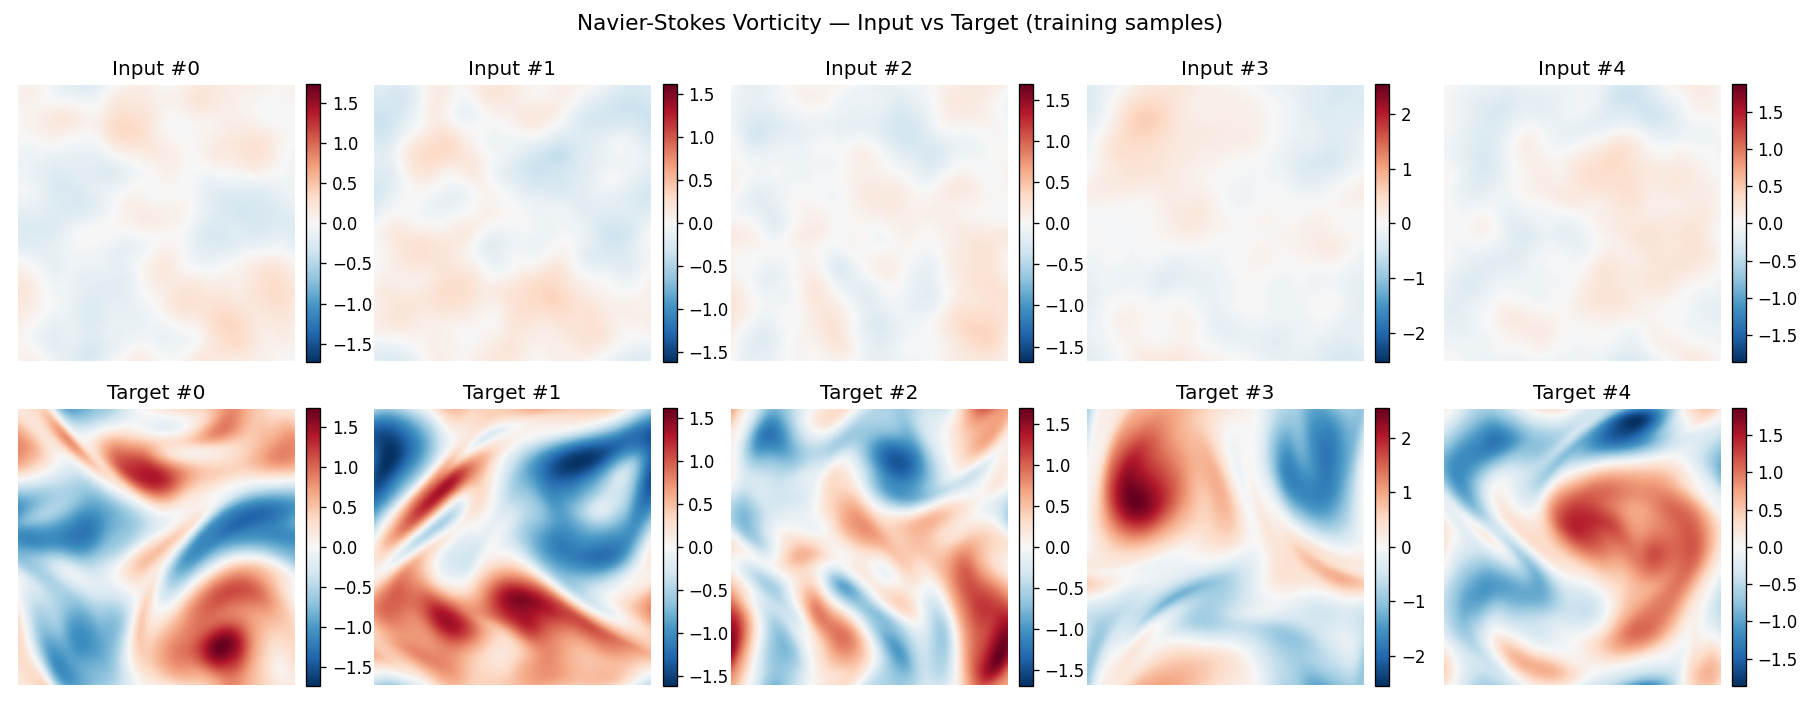
\includegraphics[width=\linewidth]{sample_pairs.png}
      {\footnotesize Vorticity snapshots: input (top) $\to$ target (bottom)}
  \end{columns}
\end{frame}

% ── 4. THE MATH — NAVIER-STOKES ───────────────────────────────────────────────
\begin{frame}{The Navier--Stokes Equations}
  2D incompressible NS in vorticity form on the unit torus $[0,1]^2$:
  \[
    \frac{\partial \omega}{\partial t} + (\mathbf{u}\cdot\nabla)\omega
    = \nu\,\nabla^2\omega + f,
    \qquad
    \omega = \nabla\times\mathbf{u},\quad \nabla\cdot\mathbf{u}=0
  \]

  \begin{columns}[t]
    \column{0.30\textwidth}
      \begin{block}{$\omega$ — Vorticity}
        \small Scalar measuring local rotation of the fluid at each grid point.
        Red = clockwise, blue = counter-clockwise.
      \end{block}
    \column{0.30\textwidth}
      \begin{block}{$(\mathbf{u}\cdot\nabla)\omega$ — Advection}
        \small Nonlinear self-interaction: the fluid's own motion shapes its future motion.
        \textbf{This causes turbulence.}
      \end{block}
    \column{0.30\textwidth}
      \begin{block}{$f$ — Kolmogorov Forcing}
        \small $f(x,y)=\sin(4\pi y)$. Sinusoidal pump that drives the system into turbulence.
        $\nu=10^{-4}$ $\Rightarrow$ Re $=10{,}000$.
      \end{block}
  \end{columns}
\end{frame}

% ── 5. DATA — INPUT TENSORS ───────────────────────────────────────────────────
\begin{frame}{Data: Input Representation \& Batching}
  \begin{columns}[t]
    \column{0.56\textwidth}
      \textbf{Dataset} --- neuraloperator Zenodo (doi:10.5281/zenodo.12825163)
      \begin{itemize}
        \item 10{,}000 training pairs \;/\; 2{,}000 test pairs
        \item Each pair: two $128\times128$ vorticity grids
      \end{itemize}
      \vspace{0.4em}
      \textbf{Tensor pipeline:}
      \begin{enumerate}
        \item Load raw pair: $\mathbf{x},\mathbf{y}\in\mathbb{R}^{128\times128}$ (\texttt{float32})
        \item FNO augments input with 2-D grid coordinates:
              $\mathbf{x}\to[\omega,g_x,g_y]\in\mathbb{R}^{3\times128\times128}$
        \item DataLoader stacks $B$ pairs $\to$ \texttt{(B,\,128,\,128)} input batch
      \end{enumerate}
      \vspace{0.4em}
      \textbf{Batching:} batch size $B=20$. Both train and test loaders use
      \texttt{num\_workers=2}, \texttt{pin\_memory=True}.

    \column{0.40\textwidth}
      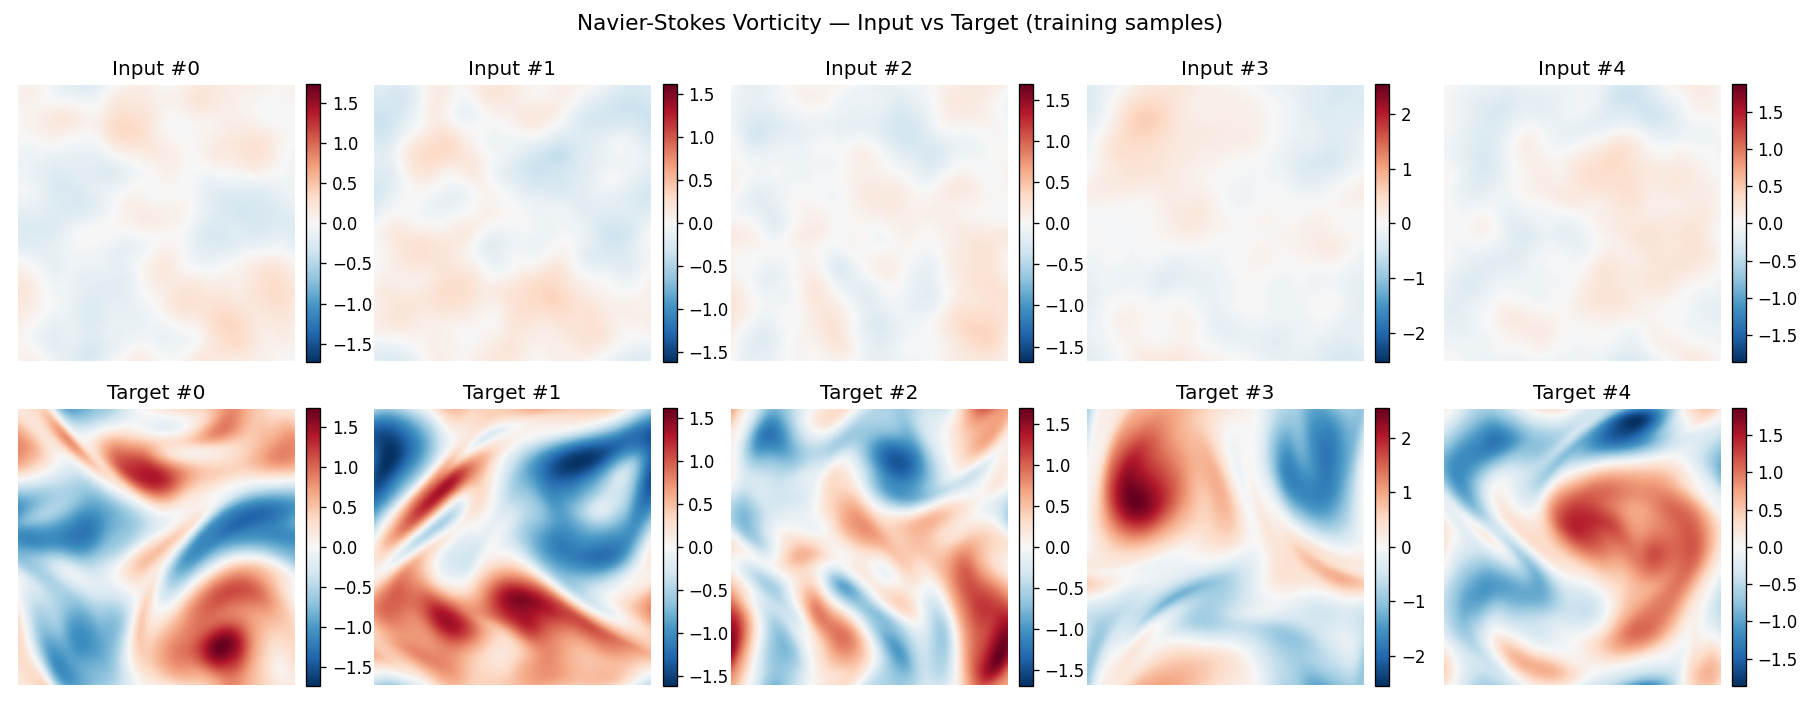
\includegraphics[width=\linewidth]{sample_pairs.png}
      \vspace{0.2em}

      {\footnotesize
      \begin{tabular}{lcc}
        \toprule
         & Input $\omega(t)$ & Target $\omega(t\!+\!1)$ \\
        \midrule
        std  & 0.15 & 0.71 \\
        range & [$-$0.76, 0.82] & [$-$3.49, 3.93] \\
        \bottomrule
      \end{tabular}
      }
  \end{columns}
\end{frame}

% ── 6. NETWORK OUTPUT ─────────────────────────────────────────────────────────
\begin{frame}{Network Output: What It Represents}
  \begin{columns}[t]
    \column{0.56\textwidth}
      Both FNO and U-Net output a single $128\times128$ tensor:
      \[
        \hat{\omega}(t+1) \in \mathbb{R}^{128\times128}
      \]
      \begin{itemize}
        \item \textbf{Regression}, not classification
        \item Each entry is a predicted vorticity value at one grid point
        \item No sigmoid or softmax --- raw real-valued output
        \item Same spatial shape as the input
      \end{itemize}
      \vspace{0.4em}
      \begin{block}{Not a probability distribution}
        The output is a \textbf{physical field} --- a prediction of the fluid state
        at the next timestep, in the same units as the input.
      \end{block}
    \column{0.40\textwidth}
      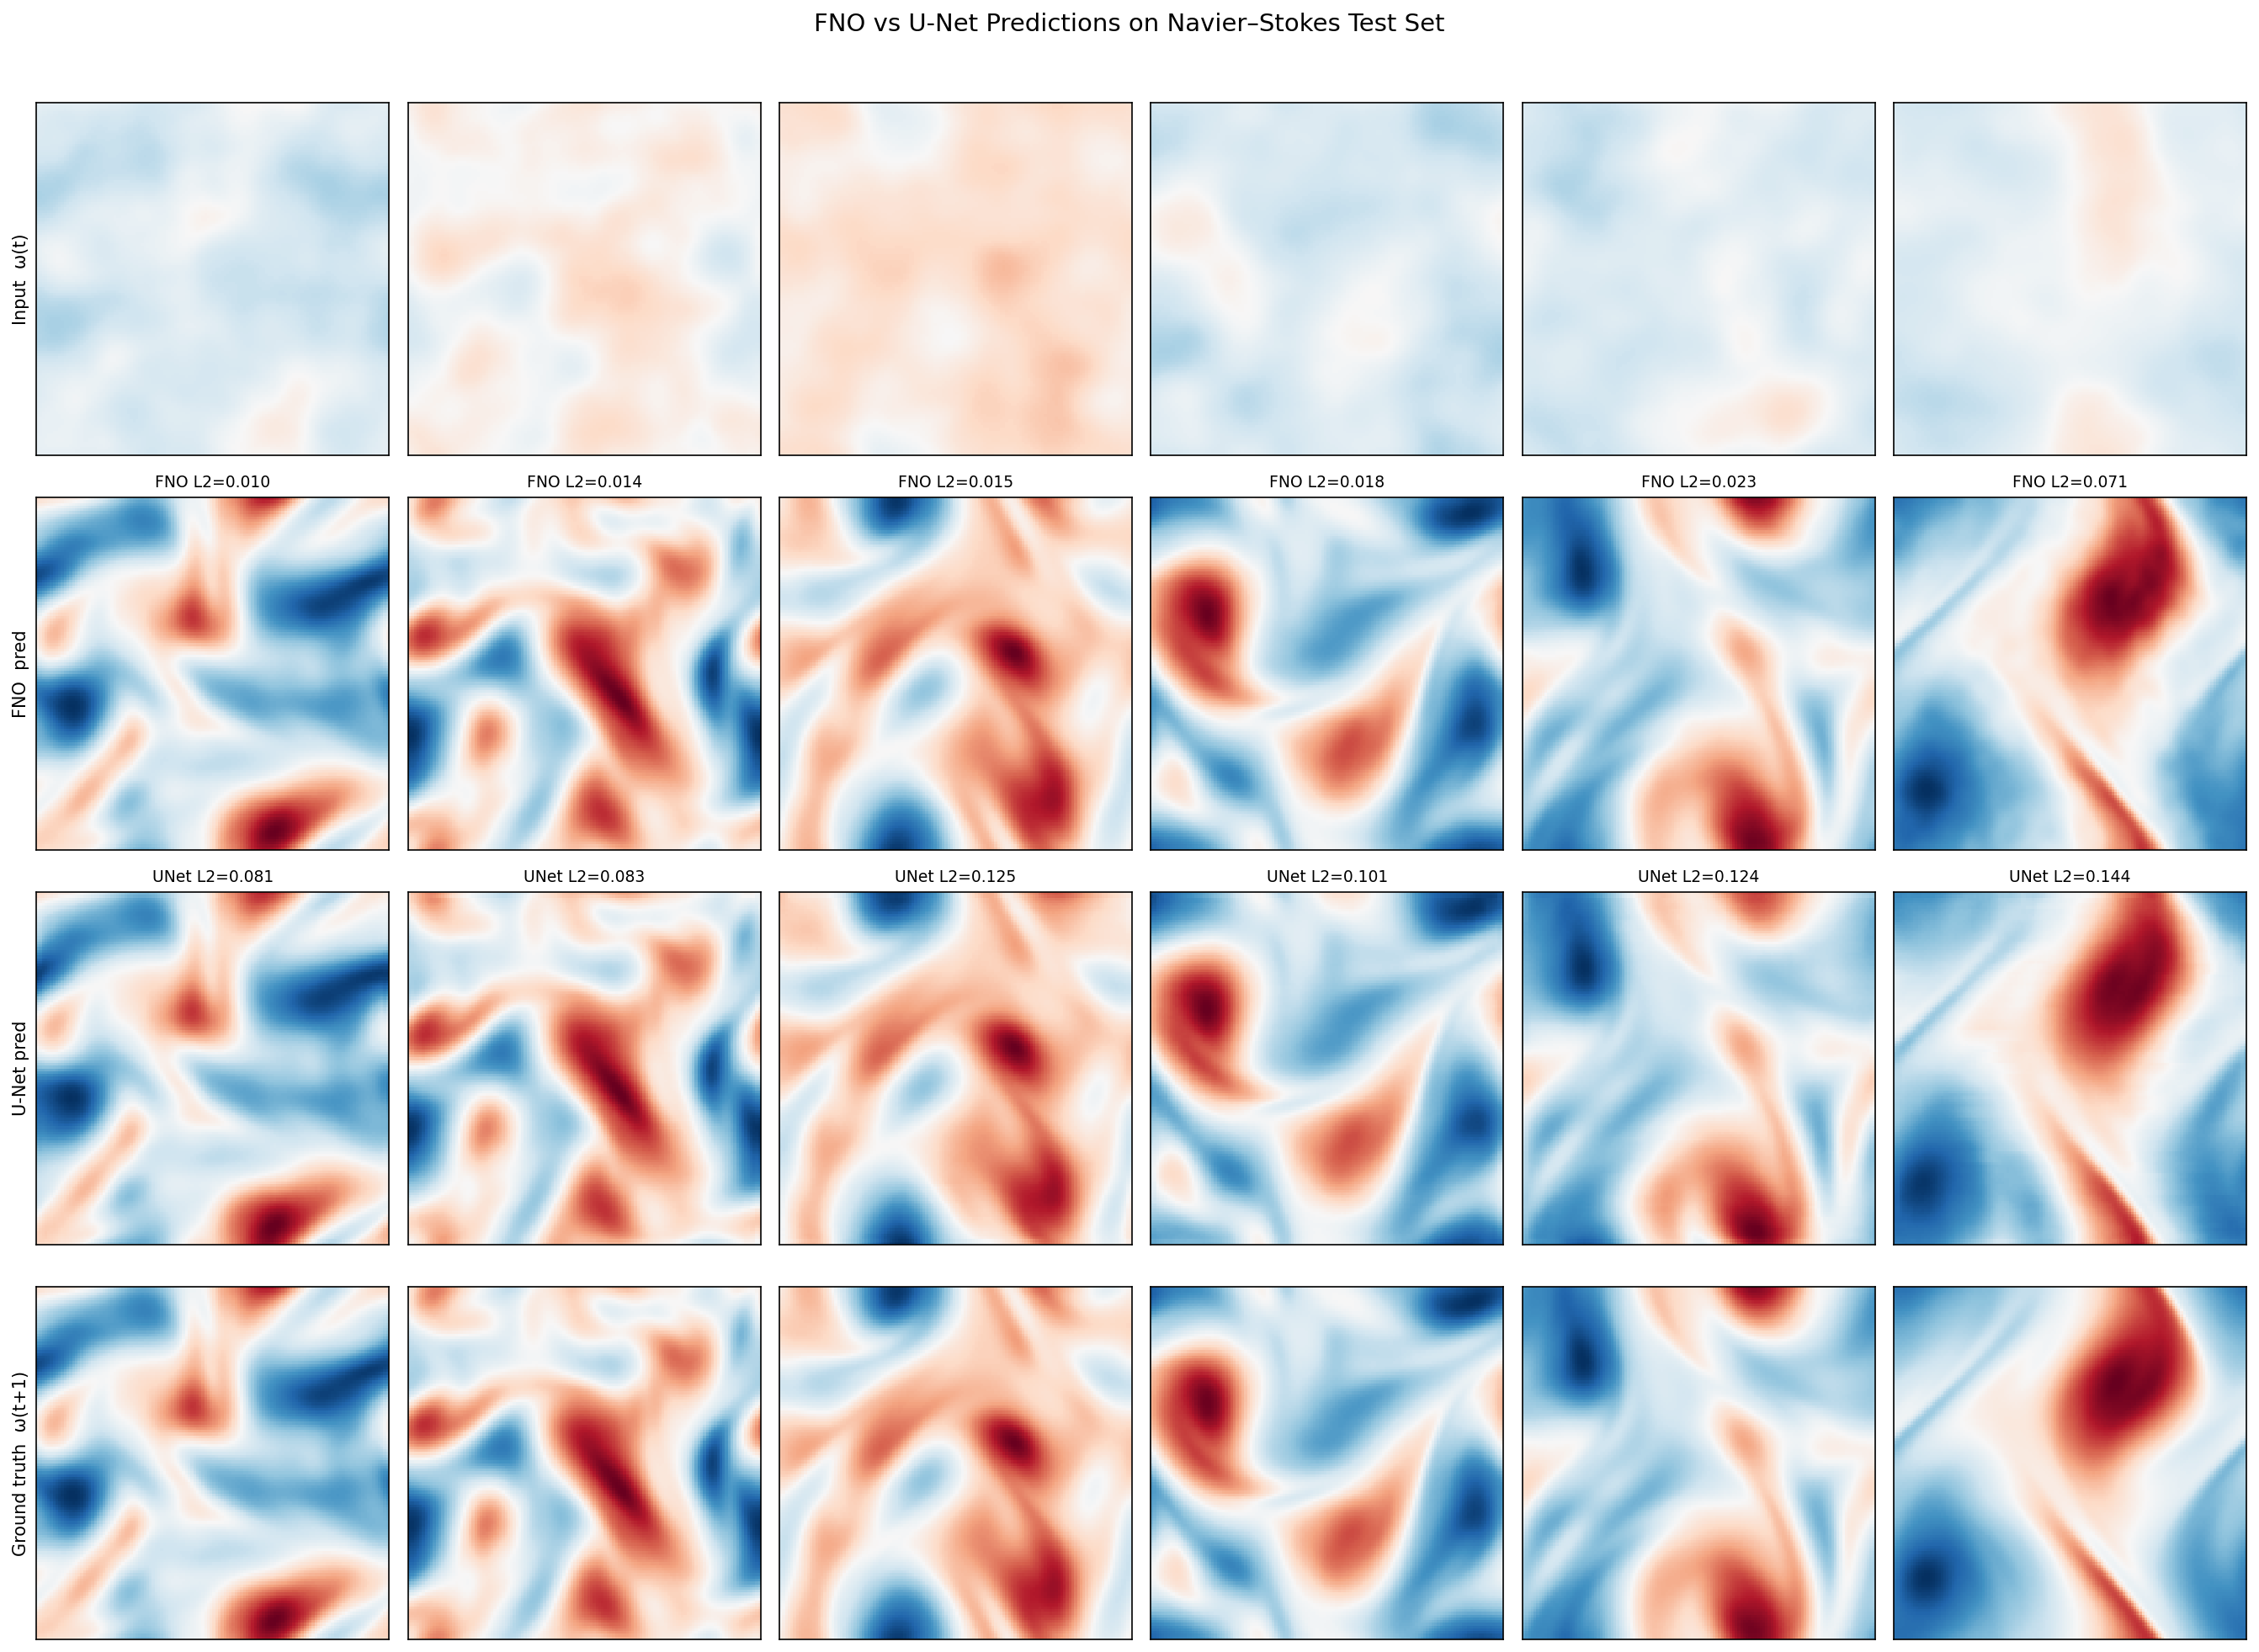
\includegraphics[width=\linewidth]{predictions.png}
      {\footnotesize Row 1: input \;|\; Row 2: FNO \;|\; Row 3: U-Net \;|\; Row 4: truth}
  \end{columns}
\end{frame}

% ── 7. LOSS FUNCTION ──────────────────────────────────────────────────────────
\begin{frame}{Loss Function: Relative $L^2$ Error}
  \begin{columns}[t]
    \column{0.52\textwidth}
      \[
        \mathcal{L}(\hat{u}, u)
        = \frac{\|\hat{u} - u\|_2}{\|u\|_2}
        = \frac{\sqrt{\sum_{i,j}(\hat{\omega}_{ij}-\omega_{ij})^2}}
               {\sqrt{\sum_{i,j}\omega_{ij}^2}}
      \]
      \vspace{0.3em}
      \begin{itemize}
        \item \textbf{Scale-invariant}: measures error as a \emph{fraction} of
              the true field's magnitude
        \item $\mathcal{L}=1.0$: prediction no better than zero (random guess)
        \item $\mathcal{L}=0.035$: error is 3.5\% of the true magnitude
        \item Averaged over all samples in a mini-batch
      \end{itemize}
      \vspace{0.3em}
      \textbf{Why not MSE?} --- MSE penalises large-amplitude samples more;
      relative $L^2$ treats all samples equally regardless of energy level.
    \column{0.44\textwidth}
      \begin{block}{Optimiser}
        Adam, lr $= 10^{-3}$, cosine annealing $\to 10^{-5}$ over 100 epochs
      \end{block}
      \vspace{0.4em}
      \begin{block}{Training budget}
        100 epochs, batch size 20\\
        NVIDIA RTX 2060 (6 GB VRAM)
      \end{block}
  \end{columns}
\end{frame}

% ── 8. FNO CORE MATH ──────────────────────────────────────────────────────────
\begin{frame}{FNO: From Integral Operators to Fourier Layers}
  A general \textbf{integral operator} acting on function $v$ is:
  \[
    (\mathcal{K}v)(x) = \int_D \kappa(x-y)\,v(y)\,dy
  \]
  By the \textbf{convolution theorem}, this equals a pointwise product in Fourier space:
  \[
    (\mathcal{K}v)(x)
    = \mathcal{F}^{-1}\!\bigl(\underbrace{R_\phi}_{\text{learned weights}}
      \cdot \underbrace{\mathcal{F}(v)}_{\text{FFT of input}}\bigr)(x)
  \]
  \begin{columns}[t]
    \column{0.48\textwidth}
      \begin{block}{Key insight}
        $R_\phi$ operates on \textbf{Fourier coefficients} (frequencies), not on
        spatial grid points. The learned operator is therefore valid at
        \textbf{any spatial resolution}.
      \end{block}
    \column{0.48\textwidth}
      \begin{block}{Implementation}
        Truncate to lowest $k=12$ modes in each dimension.
        $R_\phi \in \mathbb{C}^{C_\text{in}\times C_\text{out}\times 12\times 12}$
        applied via:
        \[
          (R_\phi\hat{v})_{b,o,x,y}
          = \sum_i R_{\phi,i,o,x,y}\,\hat{v}_{b,i,x,y}
        \]
      \end{block}
  \end{columns}
\end{frame}

% ── 9. FNO ARCHITECTURE ───────────────────────────────────────────────────────
\begin{frame}{FNO Architecture}
  \begin{columns}[t]
    \column{0.55\textwidth}
      \textbf{Full forward pass} (input $\mathbf{x}\in\mathbb{R}^{128\times128}$):
      \begin{enumerate}\small
        \item \textbf{Augment:} append 2-D grid $\to (3, 128, 128)$
        \item \textbf{Lift:} $1\times1$ conv, $3\to64$ channels
        \item \textbf{Fourier Block $\times4$:}
              \[v \leftarrow \text{GELU}\!\bigl(\mathcal{K}(v) + W_{1\times1}v\bigr)\]
        \item \textbf{Project:} $1\times1$ conv $64\to128\to1$
        \item \textbf{Output:} squeeze $\to\mathbb{R}^{128\times128}$
      \end{enumerate}
      \vspace{0.3em}
      \textbf{Bypass convolution} $W_{1\times1}$ runs in parallel with the spectral
      branch to capture local structure the truncated modes miss.

    \column{0.40\textwidth}
      \begin{block}{Config}
        \begin{tabular}{ll}
          Modes $k$ & 12 $\times$ 12 \\
          Width     & 64 channels \\
          Layers    & 4 Fourier blocks \\
          Params    & \textbf{4.7M} \\
          Activation & GELU \\
        \end{tabular}
      \end{block}
  \end{columns}
\end{frame}

% ── 10. WEIGHT INITIALISATION ─────────────────────────────────────────────────
\begin{frame}{Weight Initialisation}
  \begin{columns}[t]
    \column{0.48\textwidth}
      \begin{block}{FNO spectral weights}
        Complex weights $R_\phi^{(1)}, R_\phi^{(2)} \in
        \mathbb{C}^{C_\text{in}\times C_\text{out}\times k\times k}$
        initialised as:
        \[
          R_\phi \sim \frac{1}{C_\text{in}\cdot C_\text{out}}
                      \cdot \mathcal{U}[0,1]_\mathbb{C}
        \]
        Scaling by $1/(C_\text{in}C_\text{out})$ keeps the variance of the output
        roughly constant across layers (analogous to Xavier/Glorot).
      \end{block}
    \column{0.48\textwidth}
      \begin{block}{All Conv2d layers (FNO bypass + U-Net)}
        PyTorch default: \textbf{Kaiming uniform} (He init)
        \[
          W \sim \mathcal{U}\!\left(-\sqrt{\tfrac{6}{C_\text{in}\cdot k^2}},\;
                               \sqrt{\tfrac{6}{C_\text{in}\cdot k^2}}\right)
        \]
        Designed for ReLU/GELU activations. Keeps variance stable in deep nets.
      \end{block}
      \vspace{0.3em}
      \begin{block}{BatchNorm (U-Net only)}
        $\gamma=1$, $\beta=0$ (identity at init).
      \end{block}
  \end{columns}
\end{frame}

% ── 11. COMPARISON MODEL — U-NET ──────────────────────────────────────────────
\begin{frame}{Comparison Model: U-Net}
  \begin{columns}[t]
    \column{0.54\textwidth}
      Encoder--decoder CNN with skip connections.
      Input: $\mathbb{R}^{128\times128}\xrightarrow{\text{unsqueeze}}\mathbb{R}^{1\times128\times128}$

      \begin{itemize}\small
        \item \textbf{Encoder}: 4$\times$ (Conv$3\times3$ + BN + ReLU)$^2$ + MaxPool$\downarrow 2$
              \\channels: $1\to64\to128\to256\to512$
        \item \textbf{Bottleneck}: Conv block at $8\times8$, 1024 channels
        \item \textbf{Decoder}: 4$\times$ TransposedConv$\uparrow 2$ + skip concat + Conv block
        \item \textbf{Head}: $1\times1$ conv $\to \mathbb{R}^{128\times128}$
      \end{itemize}
      \vspace{0.3em}
      \textbf{31M parameters} --- 6.6$\times$ more than FNO.

    \column{0.42\textwidth}
      \begin{alertblock}{Key limitation}
        Fixed $3\times3$ kernels cover a specific physical length scale.
        At a new resolution the same kernel covers a \emph{different} area
        --- the learned filters lose their physical meaning.
        U-Net is \textbf{tied to its training resolution}.
      \end{alertblock}
      \vspace{0.3em}
      No physics-specific design. All structure learned purely from data.
  \end{columns}
\end{frame}

% ── 12. RESULTS TABLE ─────────────────────────────────────────────────────────
\begin{frame}{Results: Accuracy \& Speed}
  \begin{center}
  \begin{tabular}{lrrrr}
    \toprule
    Model  & Params & Rel-$L^2$$\downarrow$ & Throughput (samp/s)$\uparrow$ & Latency (ms)$\downarrow$ \\
    \midrule
    \textbf{FNO}   & 4.7M & \textbf{0.0348} & \textbf{499.2} & \textbf{2.0} \\
    U-Net & 31M  & 0.1029          & 227.0          & 4.4 \\
    \bottomrule
  \end{tabular}
  \end{center}
  \vspace{0.4em}
  \begin{columns}[t]
    \column{0.30\textwidth}
      \begin{block}{$3\times$ more accurate}
        Rel-$L^2$ 0.035 vs 0.103.\\
        Error = 3.5\% of the true\\
        field magnitude.
      \end{block}
    \column{0.30\textwidth}
      \begin{block}{$2.2\times$ faster}
        FFT-based computation on\\
        12 modes is far cheaper\\
        than full spatial convolutions.
      \end{block}
    \column{0.30\textwidth}
      \begin{block}{$6.6\times$ smaller}
        FNO stores weights for\\
        key frequencies only,\\
        not every pixel pair.
      \end{block}
  \end{columns}
\end{frame}

% ── 13. PREDICTIONS ───────────────────────────────────────────────────────────
\begin{frame}{Results: Predictions}
  \begin{center}
    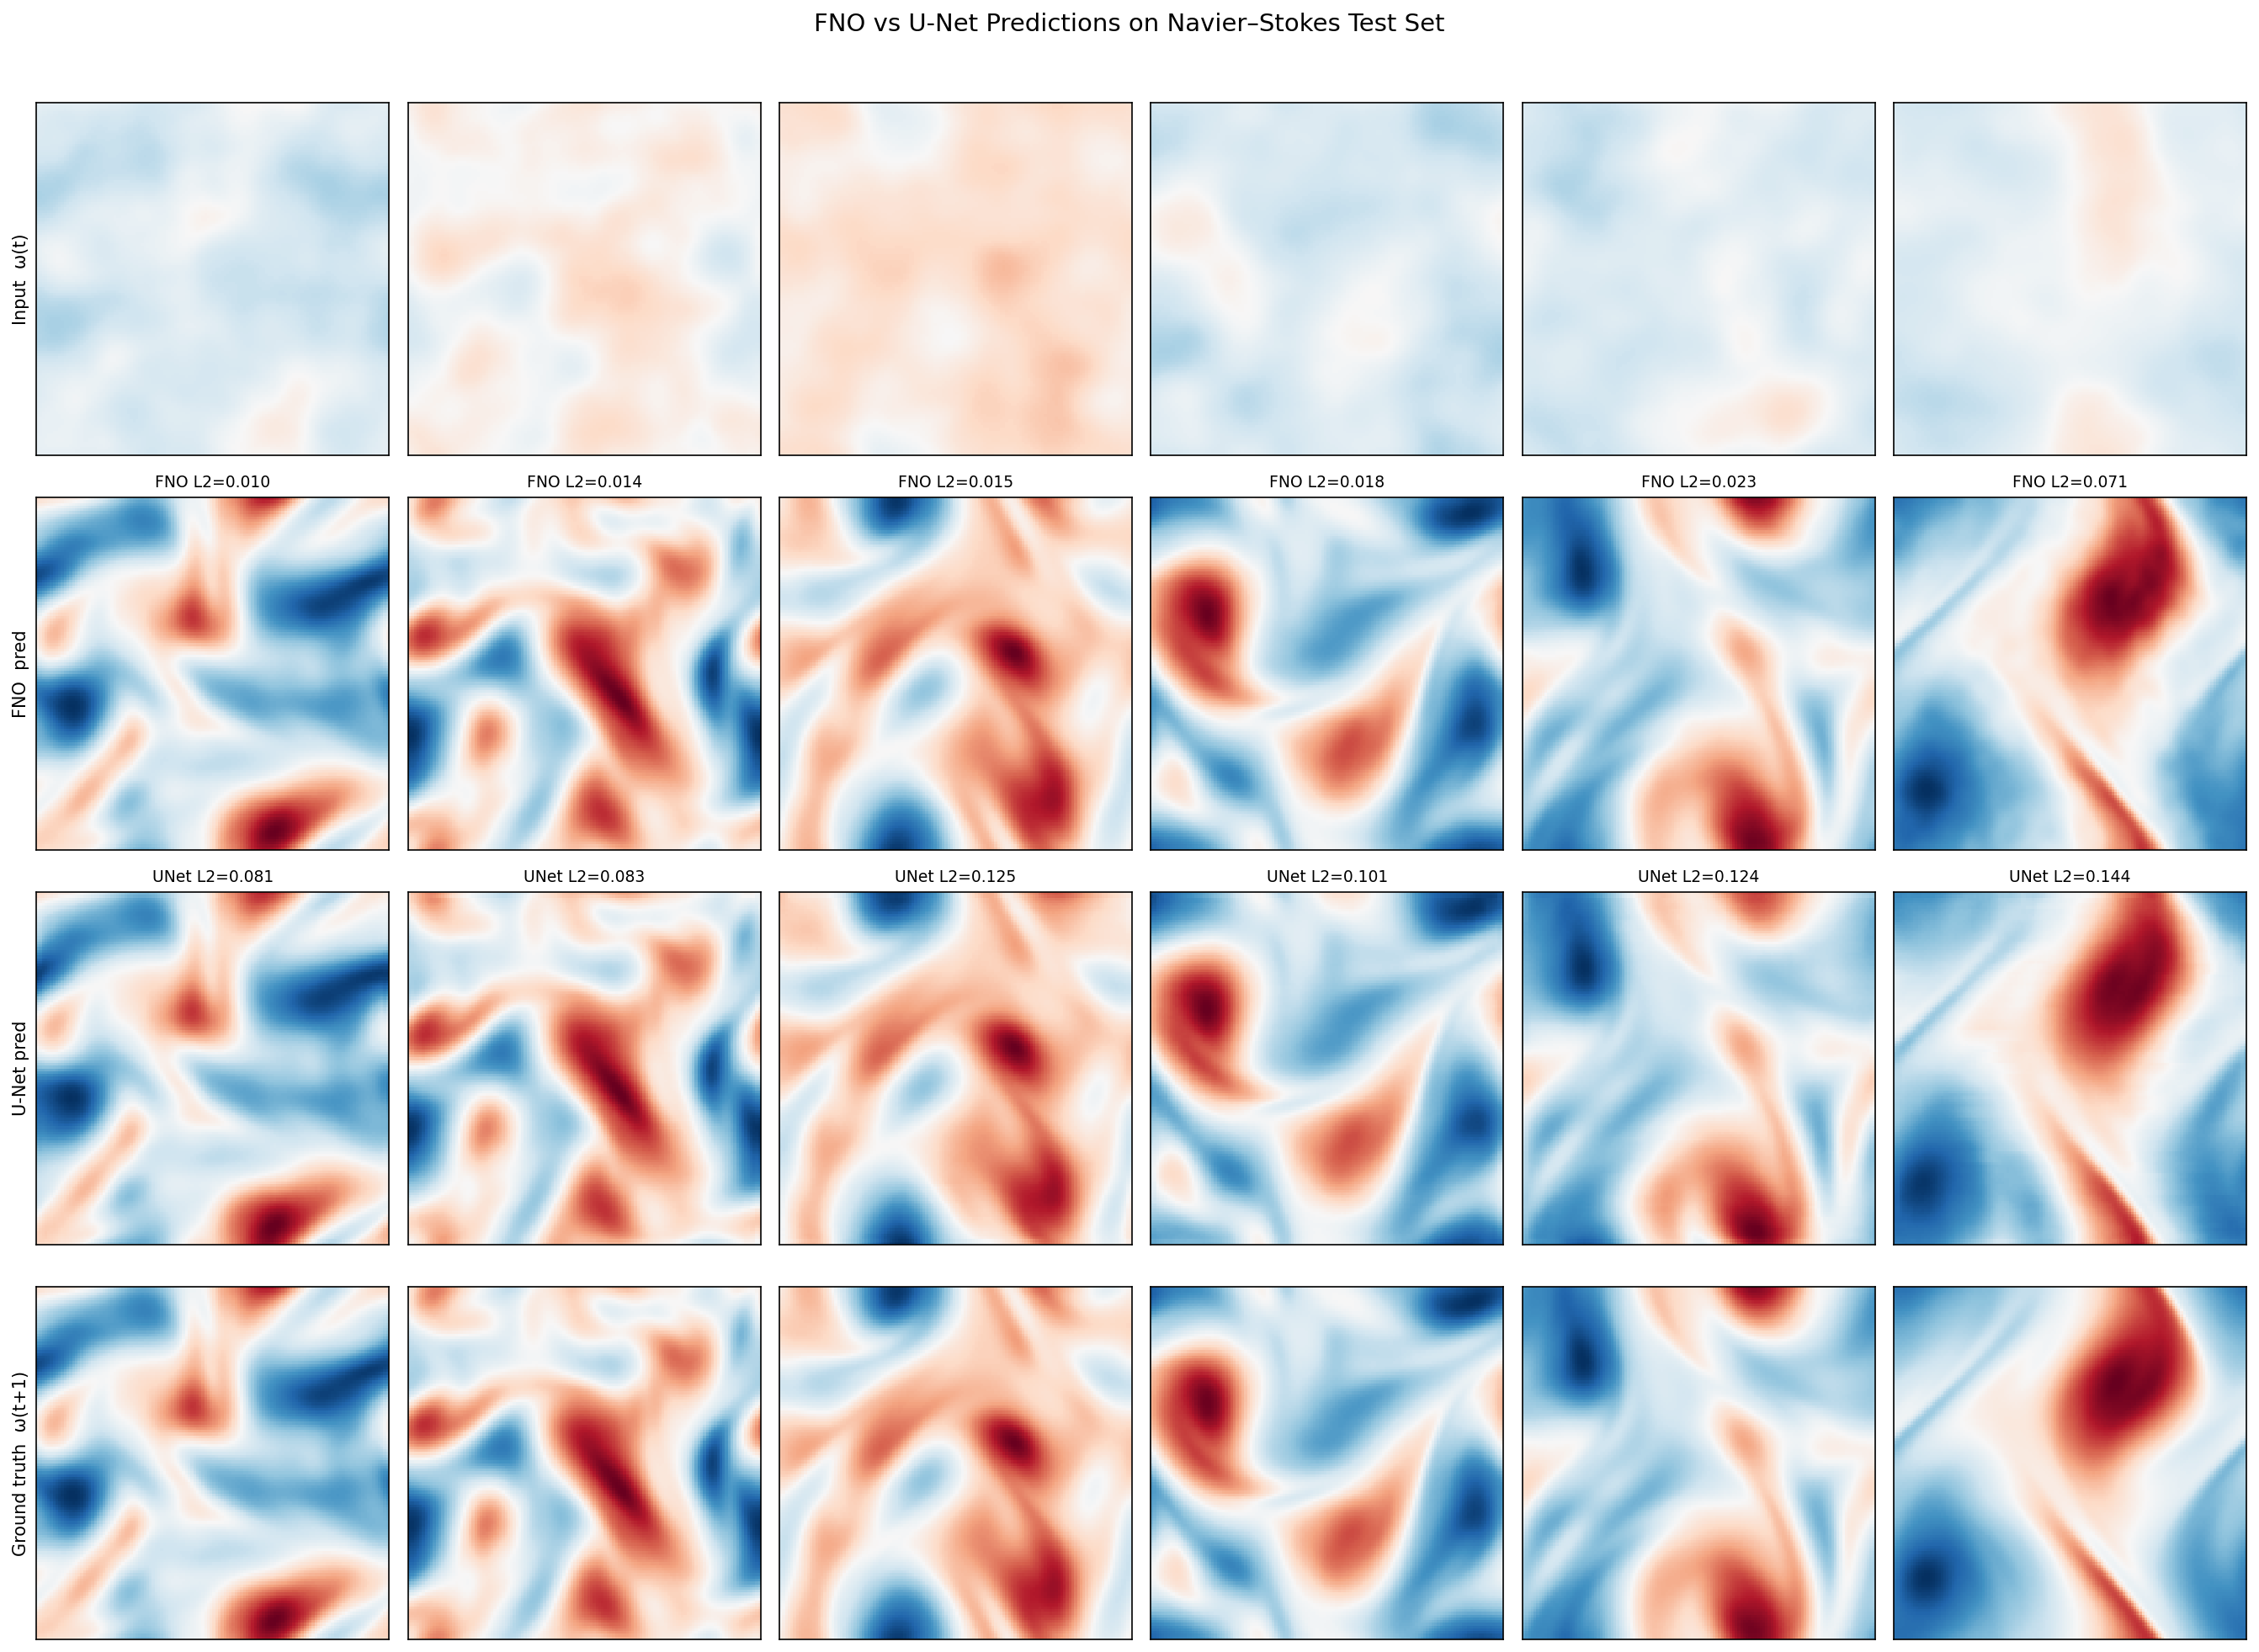
\includegraphics[width=0.95\linewidth]{predictions.png}
  \end{center}
  {\small
  Six test samples (lowest $\to$ highest FNO error). Rows: Input \;|\;
  FNO pred \;|\; U-Net pred \;|\; Ground truth. Numbers = per-sample rel-$L^2$.
  FNO matches ground truth closely; U-Net blurs vortex structure.}
\end{frame}

% ── 14. ERROR MAPS ────────────────────────────────────────────────────────────
\begin{frame}{Results: Where the Errors Are}
  \begin{columns}[t]
    \column{0.60\textwidth}
      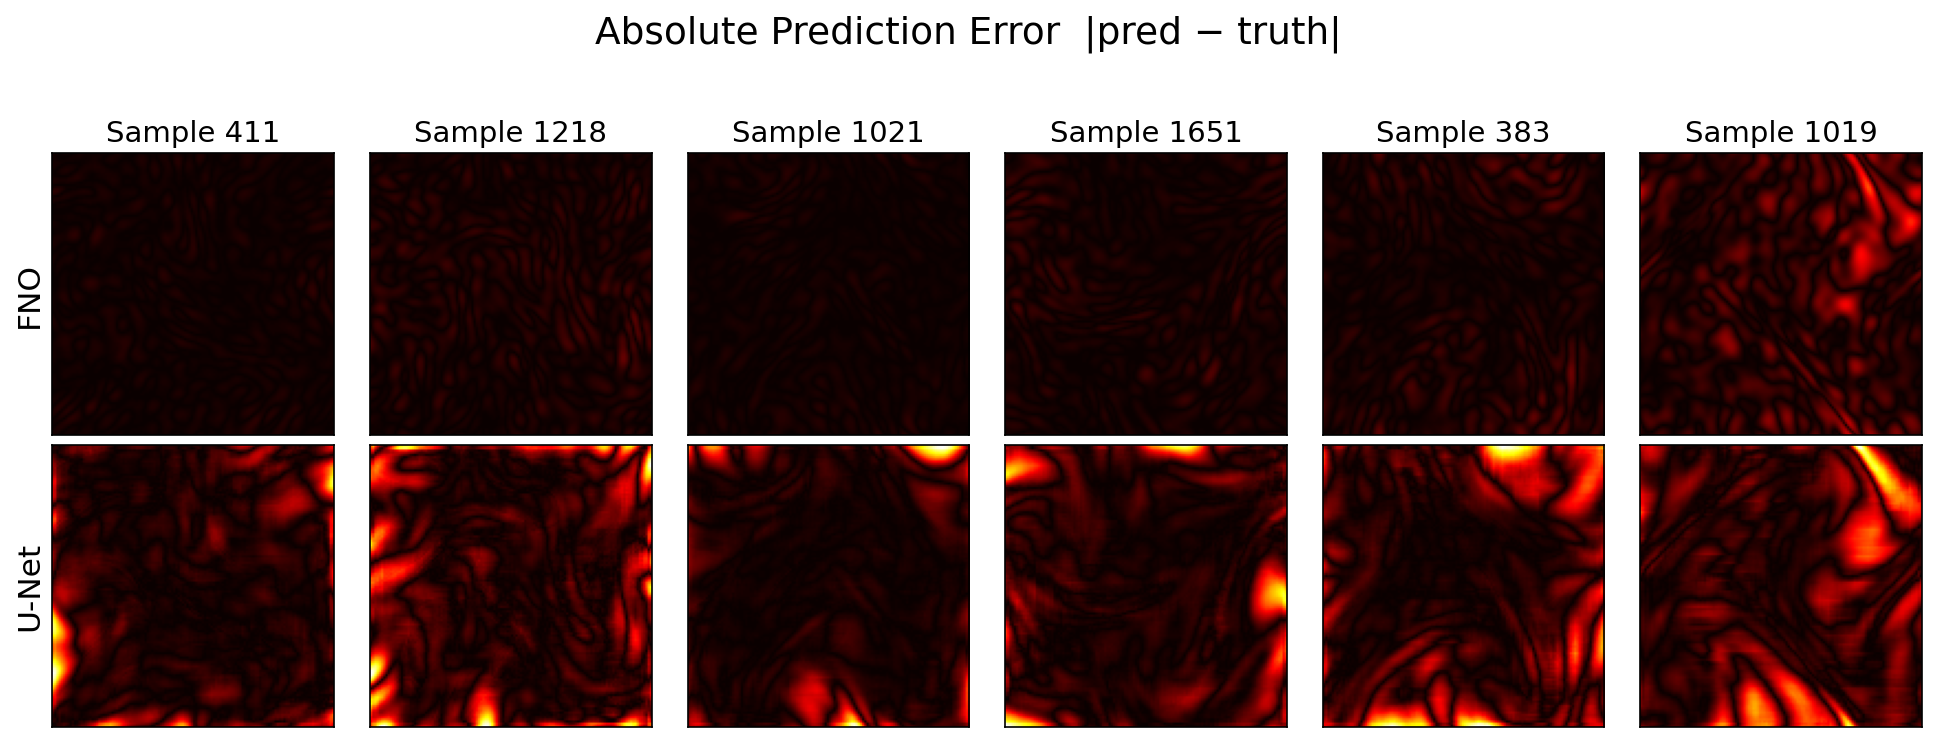
\includegraphics[width=\linewidth]{error_maps.png}
      {\footnotesize Absolute error $|\hat{\omega}-\omega|$. Top: FNO. Bottom: U-Net.
      Hot colormap --- brighter = larger error.}
    \column{0.36\textwidth}
      \begin{block}{FNO}
        Errors small and diffuse, spread evenly across the domain.
      \end{block}
      \vspace{0.4em}
      \begin{alertblock}{U-Net}
        Errors \textbf{concentrated at vortex boundaries} --- exactly where the
        physics is most nonlinear and the gradient changes most rapidly.
      \end{alertblock}
  \end{columns}
\end{frame}

% ── 15. SUPER-RESOLUTION ──────────────────────────────────────────────────────
\begin{frame}{Zero-Shot Super-Resolution}
  \textit{Both models trained only on $128\times128$. Evaluated at unseen resolutions with no retraining.}
  \vspace{0.2em}
  \begin{columns}[t]
    \column{0.38\textwidth}
      \begin{center}
      \begin{tabular}{lcc}
        \toprule
        Resolution & FNO & U-Net \\
        \midrule
        $64\times64$  & \textbf{0.019} & 0.476 \\
        $128\times128$ & \textbf{0.019} & 0.103 \\
        $256\times256$ & \textbf{0.019} & 0.594 \\
        \bottomrule
      \end{tabular}
      \end{center}
      \vspace{0.3em}
      FNO error: \textbf{identical} at all 3 resolutions.\\
      U-Net at $256^2$: barely better than a random guess ($\mathcal{L}=1.0$).
    \column{0.58\textwidth}
      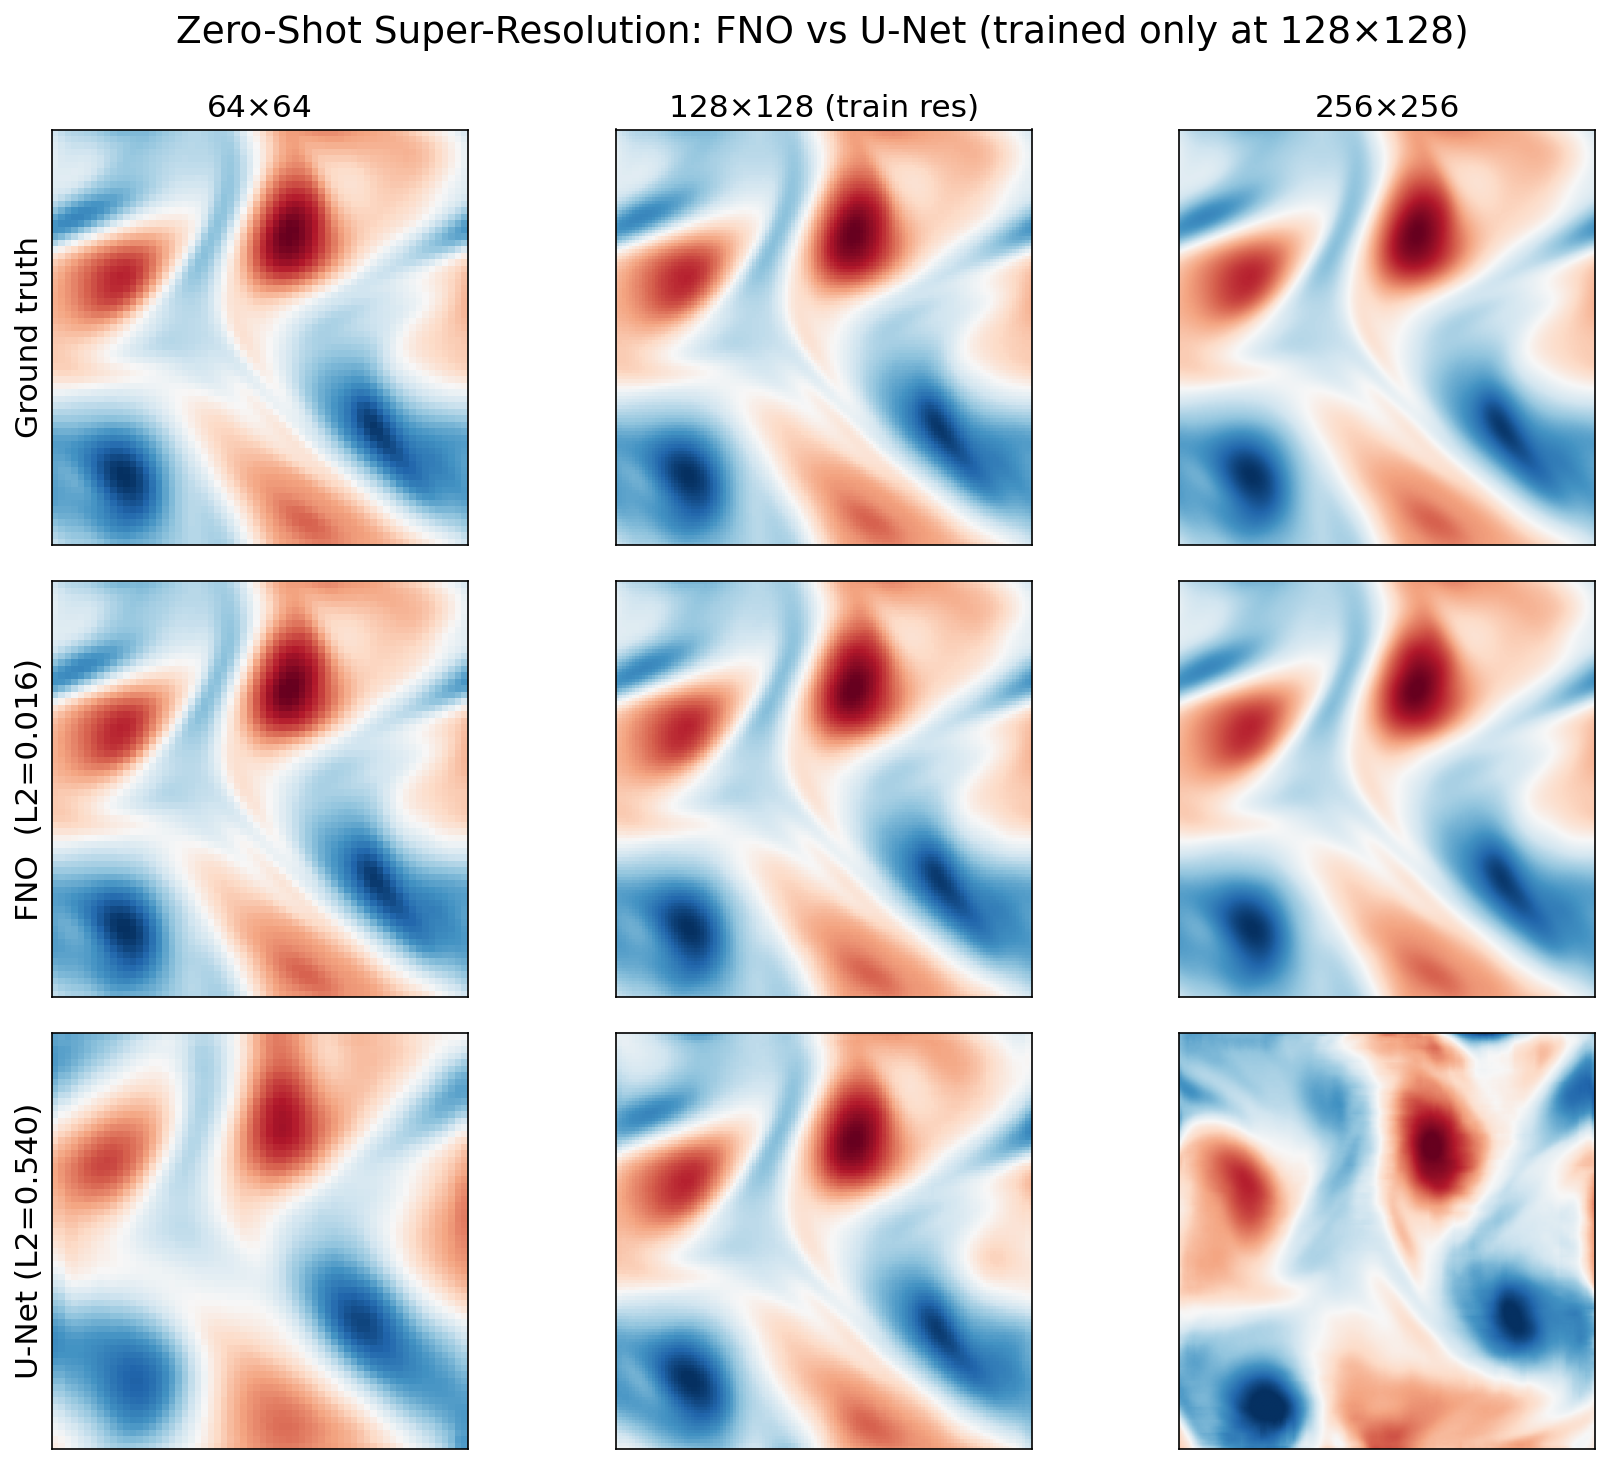
\includegraphics[width=\linewidth]{super_res.png}
      {\footnotesize Cols: $64^2$ \;|\; $128^2$ \;|\; $256^2$. Rows: truth / FNO / U-Net.}
  \end{columns}
\end{frame}

% ── 16. WHY FNO WINS ──────────────────────────────────────────────────────────
\begin{frame}{Why FNO Wins: Inductive Bias}
  \begin{columns}[t]
    \column{0.48\textwidth}
      \begin{block}{Global vs.\ local}
        NS dynamics are \textbf{global}: a vortex anywhere changes pressure
        everywhere via the Poisson equation.
        \begin{itemize}
          \item FNO: FFT sees the entire domain at once
          \item U-Net: $3\times3$ kernels see a local patch; many layers needed
                to propagate long-range information
        \end{itemize}
      \end{block}
    \column{0.48\textwidth}
      \begin{block}{Resolution independence}
        FNO learns weights $R_\phi$ for Fourier modes.\\
        Mode $k$ = ``swirl repeating $k$ times'' ---
        same physical meaning at any grid spacing.\\[4pt]
        U-Net's $3\times3$ kernel at $128^2$ covers physical scale $3/128$.\\
        At $256^2$ the same kernel covers $3/256$ ---
        \textbf{half the physical area}. Every filter changes meaning.
      \end{block}
  \end{columns}
  \vspace{0.4em}
  \begin{alertblock}{Broader lesson}
    Architecture-level \textbf{inductive bias} (encoding the right physics into the model design)
    outperforms raw parameter count when the bias matches the problem structure.
  \end{alertblock}
\end{frame}

% ── 17. CONCLUSION ────────────────────────────────────────────────────────────
\begin{frame}{Conclusion}
  \begin{columns}[t]
    \column{0.54\textwidth}
      \textbf{What we showed:}
      \begin{itemize}
        \item Neural networks can learn to predict fluid dynamics directly from data
        \item FNO: \textbf{$3\times$ lower error, $2.2\times$ faster, $6.6\times$ smaller} than U-Net
        \item FNO error flat across all resolutions; U-Net collapses at unseen sizes
        \item A model designed to match the physics beats a larger generic one
      \end{itemize}
    \column{0.42\textwidth}
      \textbf{Limitations:}
      \begin{itemize}
        \item Single viscosity $\nu=10^{-4}$ only
        \item Single-step prediction --- errors compound over rollout
        \item Super-resolution ground truth is approximate (bilinear upsample)
      \end{itemize}
      \vspace{0.4em}
      \textbf{Code \& data:}\\
      {\footnotesize\texttt{github.com/baldihug/\\COMP395-Final-Group-Project}}
  \end{columns}
  \vspace{0.4em}
  \begin{block}{References}
    \footnotesize
    Li et al.\ (2021). \textit{Fourier Neural Operator for Parametric PDEs.} ICLR.
    \href{https://arxiv.org/abs/2010.08895}{arXiv:2010.08895} \quad
    Ronneberger et al.\ (2015). \textit{U-Net.} MICCAI. \quad
    Dataset: doi:10.5281/zenodo.12825163
  \end{block}
\end{frame}

\end{document}
